%!TEX root = ../paper.tex

\section{Risk Benefit Assessments of Various Technologies}
\label{sec:riskben-appendix} 

\begin{table}[h!!!!]
\begin{center}
\small
\begin{tabular}{| p{2cm} | p{1cm} | p{1cm} | p{1cm} | c |}
\hline
Technology & Q1 &  Median & Q3 & Distribution  \\ 
\hline
Location Tracking & 10.0 & 10.0 & 20.0 & 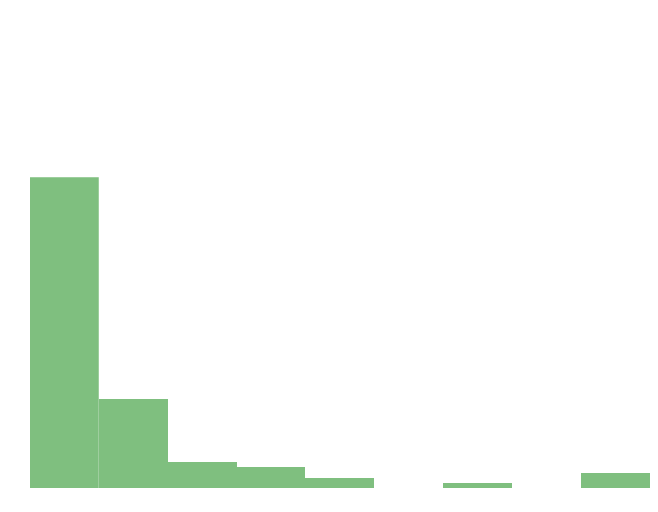
\includegraphics[width = 2cm, height = 0.5cm]{tex-inputs/table-images/locationtrackingrisk} \\ 
Speech To Text & 10.0 & 10.0 & 10.0 & 
\includegraphics[width = 2cm, height = 0.5cm]{tex-inputs/table-images/speechtotextrisk} \\ 
Discreet Microphone & 10.0 & 10.0 & 20.0 & 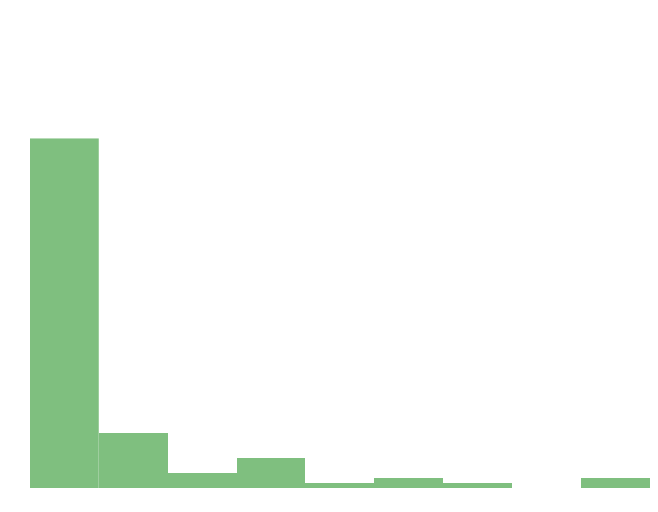
\includegraphics[width = 2cm, height = 0.5cm]{tex-inputs/table-images/discreetmicrophonerisk} \\ 
Smartwatches & 10.0 & 10.0 & 10.0 & 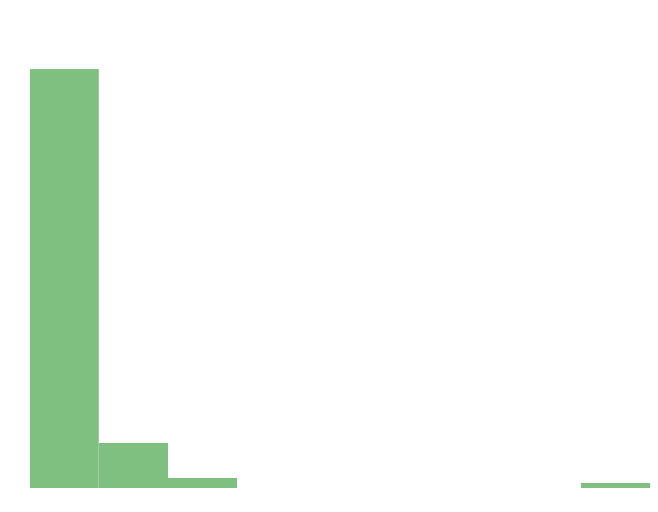
\includegraphics[width = 2cm, height = 0.5cm]{tex-inputs/table-images/smartwatchesrisk} \\ 
Language Detection & 10.0 & 10.0 & 10.0 & 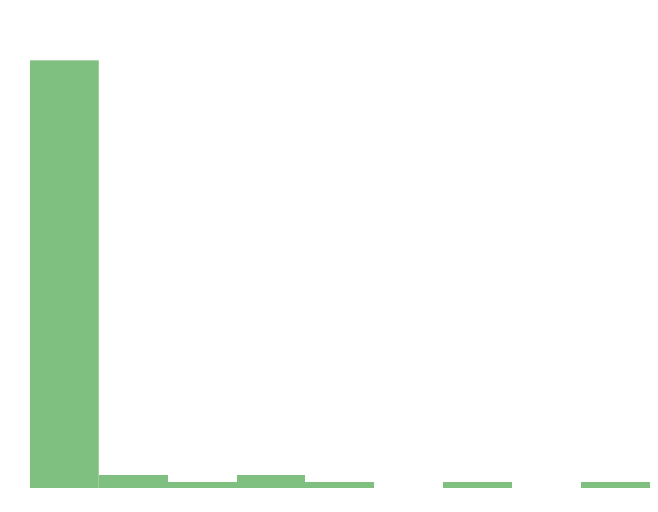
\includegraphics[width = 2cm, height = 0.5cm]{tex-inputs/table-images/languagedetectionrisk} \\ 
Laptops & 10.0 & 10.0 & 15.0 & 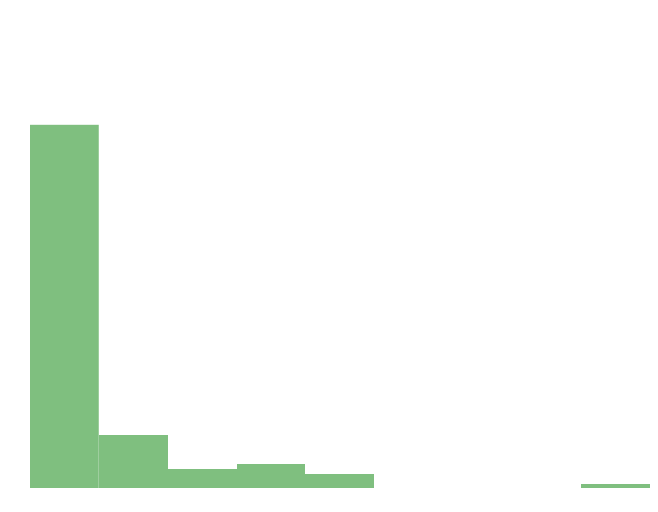
\includegraphics[width = 2cm, height = 0.5cm]{tex-inputs/table-images/laptopsrisk} \\ 
Smartphones & 10.0 & 10.0 & 20.0 & 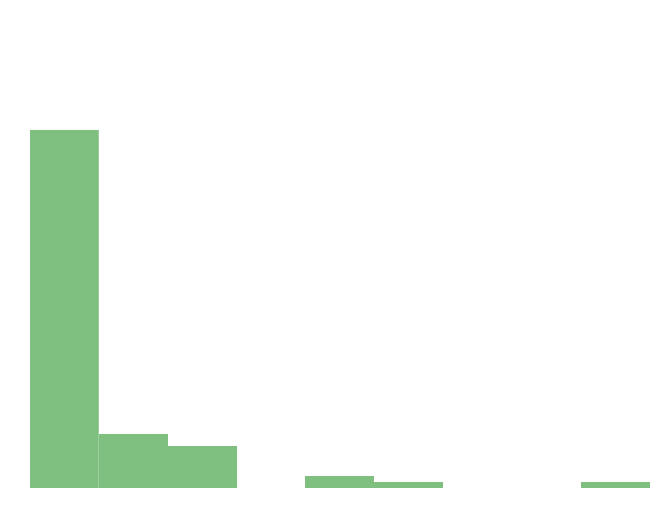
\includegraphics[width = 2cm, height = 0.5cm]{tex-inputs/table-images/smartphonesrisk} \\ 
Google Glass & 10.0 & 10.0 & 20.0 & 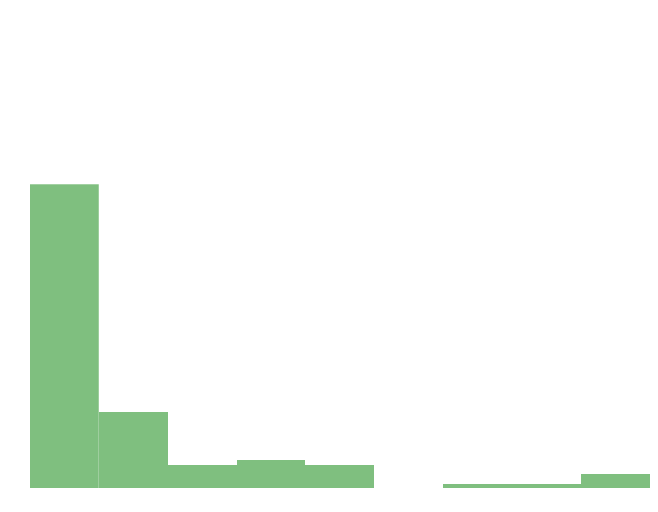
\includegraphics[width = 2cm, height = 0.5cm]{tex-inputs/table-images/googleglassrisk} \\ 
Cubetastic & 10.0 & 10.0 & 30.0 & 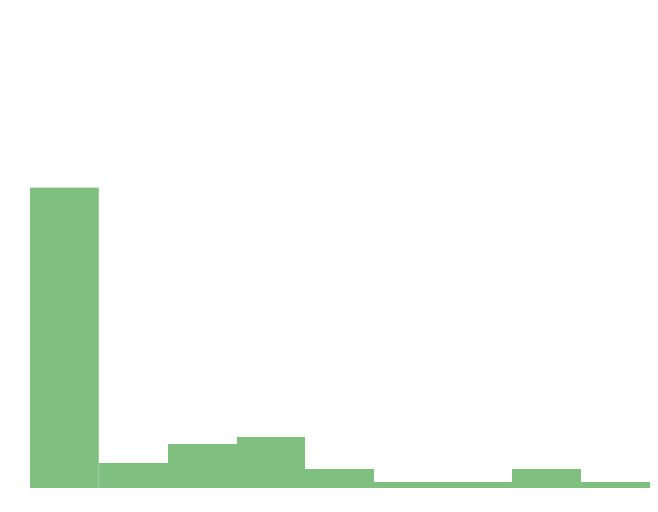
\includegraphics[width = 2cm, height = 0.5cm]{tex-inputs/table-images/cubetasticrisk} \\ 
Gender Detection & 10.0 & 10.0 & 13.5 & 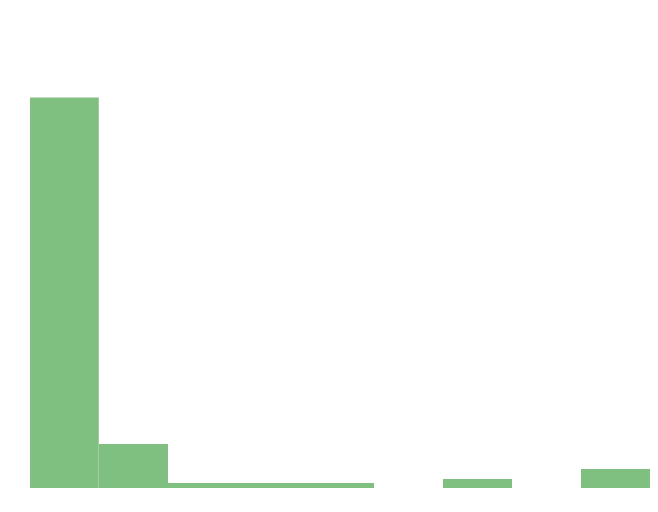
\includegraphics[width = 2cm, height = 0.5cm]{tex-inputs/table-images/genderdetectionrisk} \\ 
Voice Recognition & 10.0 & 10.0 & 15.0 & 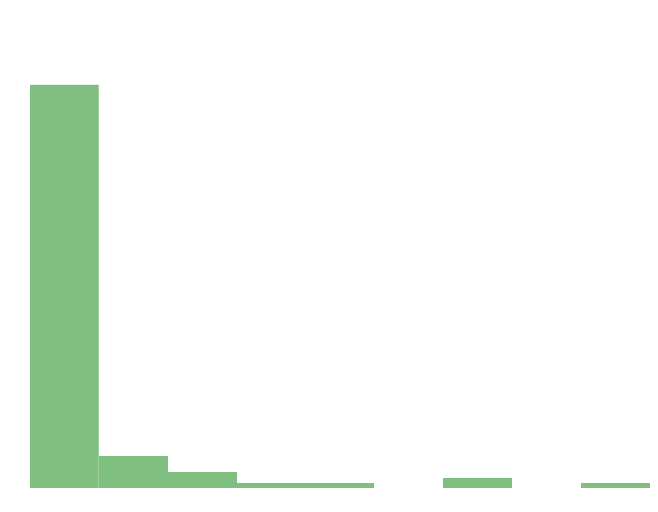
\includegraphics[width = 2cm, height = 0.5cm]{tex-inputs/table-images/voicerecognitionrisk} \\ 
Voice Based Emotion Detection & 10.0 & 10.0 & 15.0 & 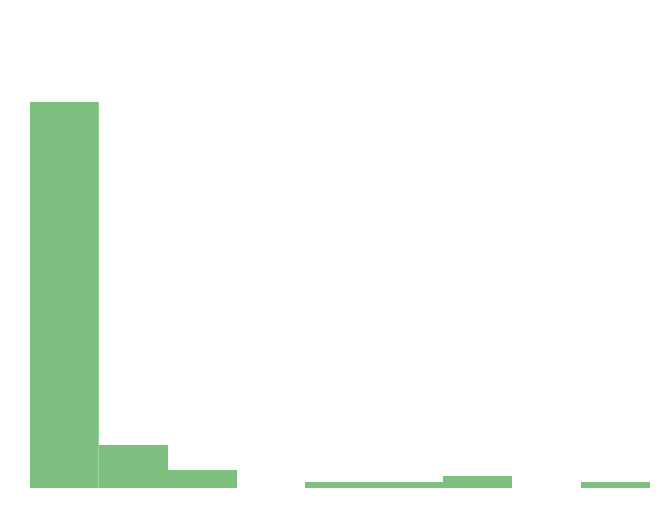
\includegraphics[width = 2cm, height = 0.5cm]{tex-inputs/table-images/voicebasedemotiondetectionrisk} \\ 
Fitness Trackers & 10.0 & 10.0 & 10.0 & 
\includegraphics[width = 2cm, height = 0.5cm]{tex-inputs/table-images/fitnesstrackersrisk} \\ 
Age Detection & 10.0 & 10.0 & 15.0 & 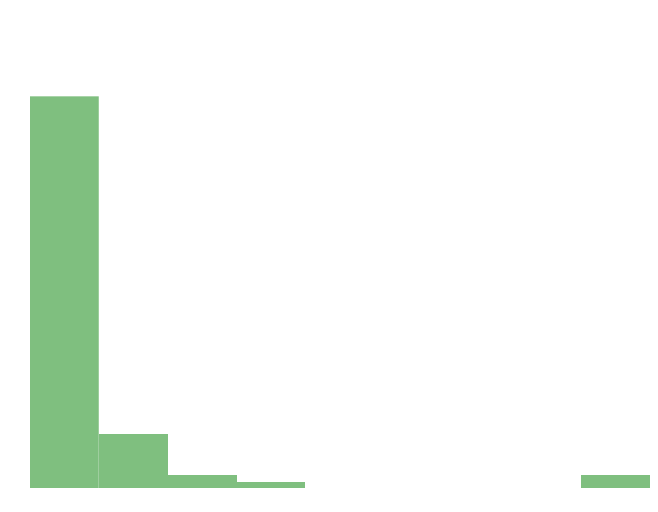
\includegraphics[width = 2cm, height = 0.5cm]{tex-inputs/table-images/agedetectionrisk} \\ 
Facial Detection & 10.0 & 10.0 & 25.0 & 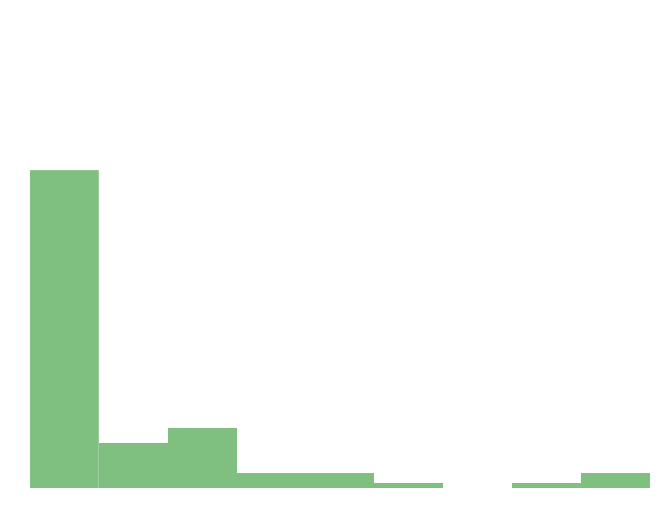
\includegraphics[width = 2cm, height = 0.5cm]{tex-inputs/table-images/facialdetectionrisk} \\ 
Email & 10.0 & 10.0 & 18.0 & 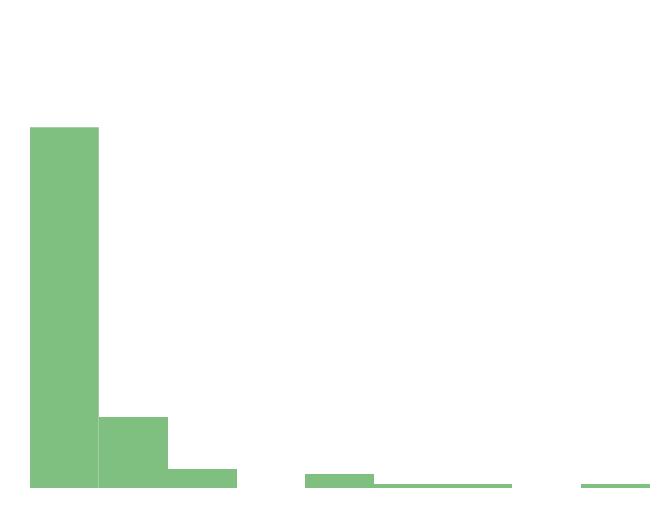
\includegraphics[width = 2cm, height = 0.5cm]{tex-inputs/table-images/emailrisk} \\ 
Heart Rate Detection & 10.0 & 10.0 & 10.0 & 
\includegraphics[width = 2cm, height = 0.5cm]{tex-inputs/table-images/heartratedetectionrisk} \\ 
Discreet Video Camera & 12.0 & 10.0 & 30.0 & 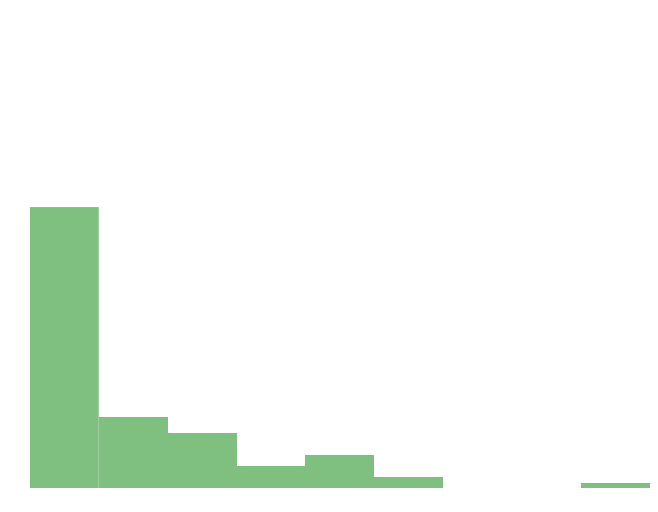
\includegraphics[width = 2cm, height = 0.5cm]{tex-inputs/table-images/discreetvideocamerarisk} \\ 
Internet & 15.0 & 10.0 & 31.0 & 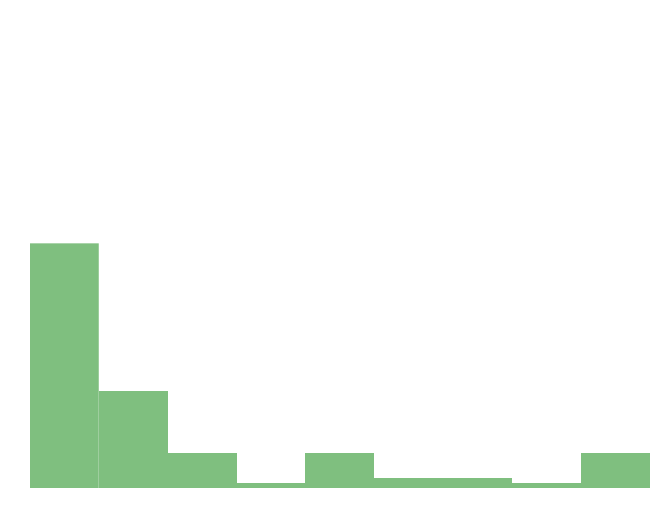
\includegraphics[width = 2cm, height = 0.5cm]{tex-inputs/table-images/internetrisk} \\ 
Facial Recognition & 17.0 & 10.0 & 30.0 & 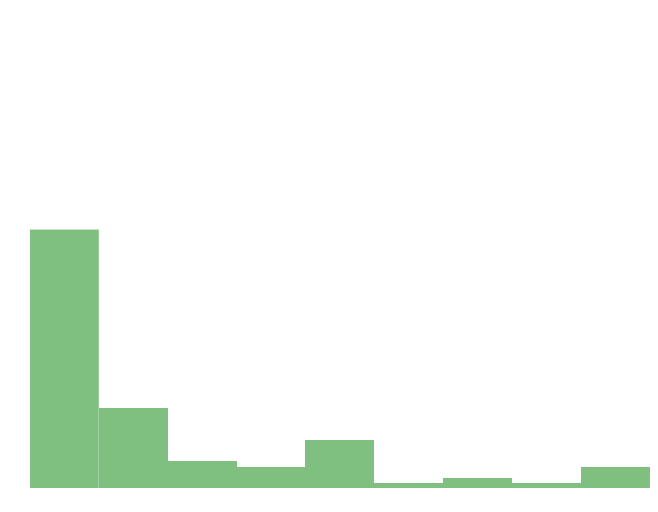
\includegraphics[width = 2cm, height = 0.5cm]{tex-inputs/table-images/facialrecognitionrisk} \\ 
Lawnmower & 20.0 & 12.0 & 30.0 & 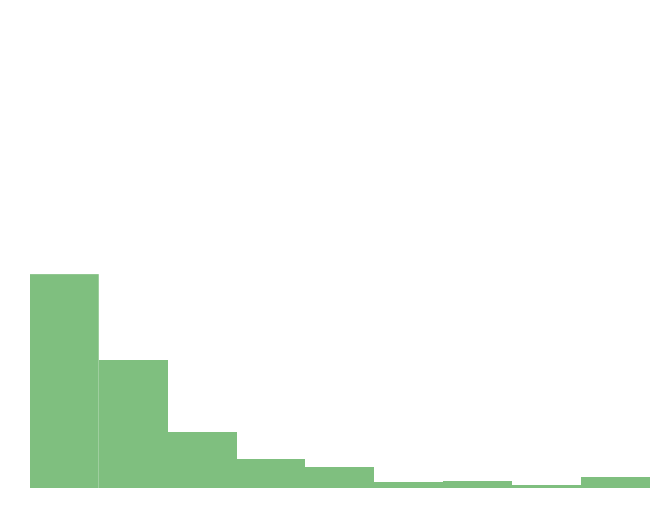
\includegraphics[width = 2cm, height = 0.5cm]{tex-inputs/table-images/LawnmowerRisk} \\ 
Electricity & 25.0 & 15.0 & 40.0 & 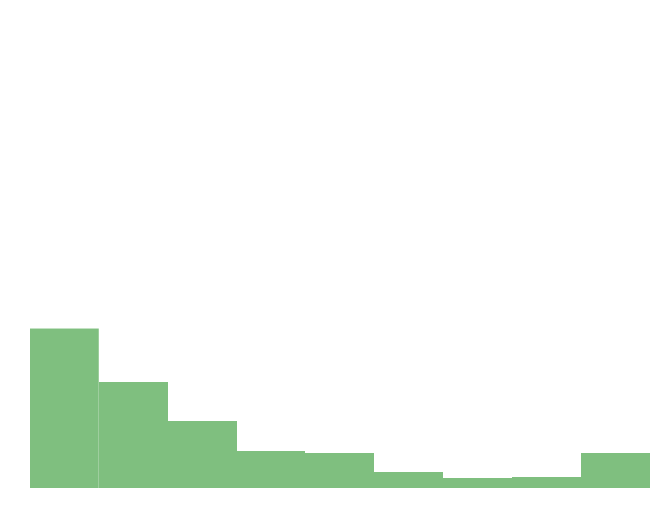
\includegraphics[width = 2cm, height = 0.5cm]{tex-inputs/table-images/ElectricityRisk} \\ 
Motorcycle & 45.0 & 27.0 & 70.0 & 
\includegraphics[width = 2cm, height = 0.5cm]{tex-inputs/table-images/MotorcycleRisk} \\ 
Handgun & 60.0 & 40.0 & 100.0 & 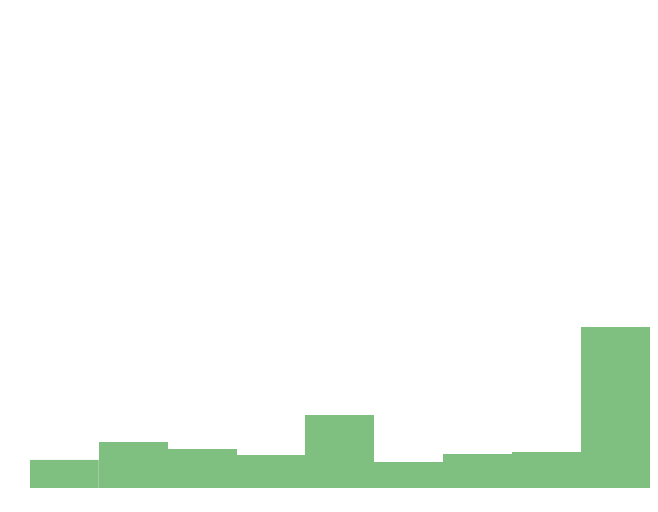
\includegraphics[width = 2cm, height = 0.5cm]{tex-inputs/table-images/HandgunRisk} \\ 
\hline
\end{tabular}
\caption{Risk rankings in response to the Fischoff-style prompt for various technologies and capabilities.Most technologies are capabilities with respect to wearable devices. Calibration technologies were electricity, guns, lawnmowers, and motorcycles. Wearable technologies included the Google Glass and the Cubetastic3000. Other specific technologies, such as internet, email, laptops, and smartphones, were also asked.}
\label{risk}
\end{center}
\end{table}

\begin{table}[h!!!!!]
\begin{center}
\small
\begin{tabular}{| p{2cm} | p{1cm} | p{1cm} | p{1cm} | c |}
\hline
Technology & Q1 &  Median & Q3 & Distribution  \\ 
\hline
Gender Detection & 10.0 & 10.0 & 15.0 & 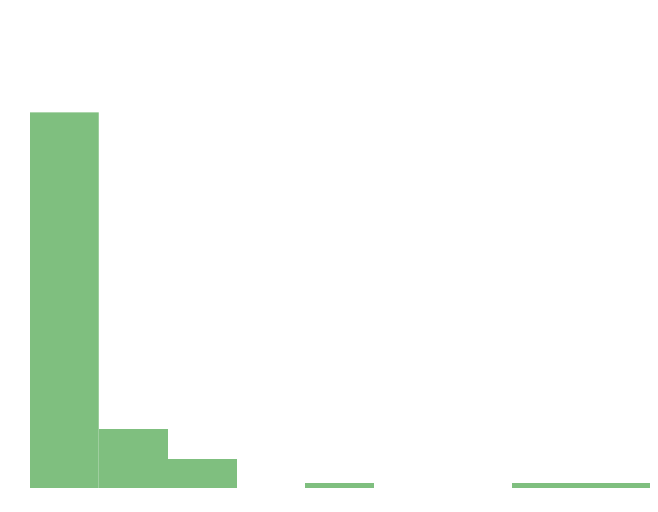
\includegraphics[width = 2cm, height = 0.5cm]{tex-inputs/table-images/genderdetectionben} \\ 
Age Detection & 12.0 & 10.0 & 22.0 & 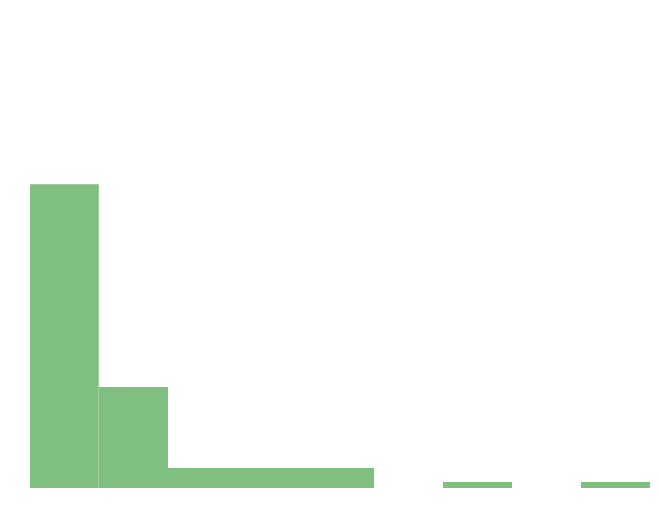
\includegraphics[width = 2cm, height = 0.5cm]{tex-inputs/table-images/agedetectionben} \\ 
Discreet Microphone & 15.0 & 10.0 & 20.0 & 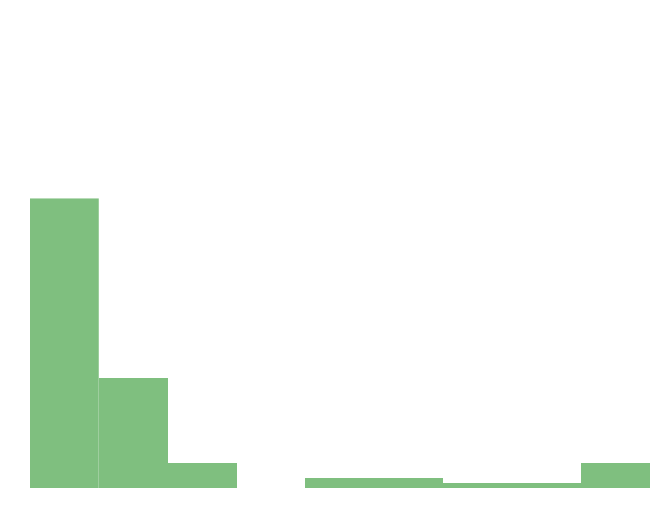
\includegraphics[width = 2cm, height = 0.5cm]{tex-inputs/table-images/discreetmicrophoneben} \\ 
Cubetastic & 15.0 & 10.0 & 30.0 & 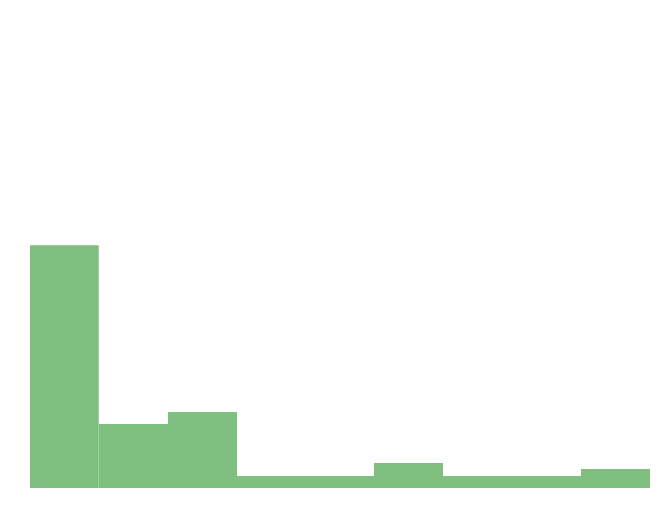
\includegraphics[width = 2cm, height = 0.5cm]{tex-inputs/table-images/cubetasticben} \\ 
Fitness Trackers & 18.5 & 10.0 & 30.0 & 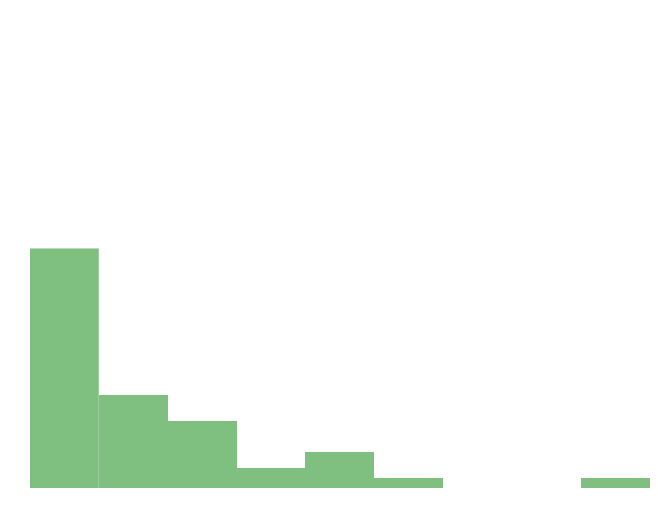
\includegraphics[width = 2cm, height = 0.5cm]{tex-inputs/table-images/fitnesstrackersben} \\ 
Voice Based Emotion Detection & 20.0 & 10.0 & 30.0 & 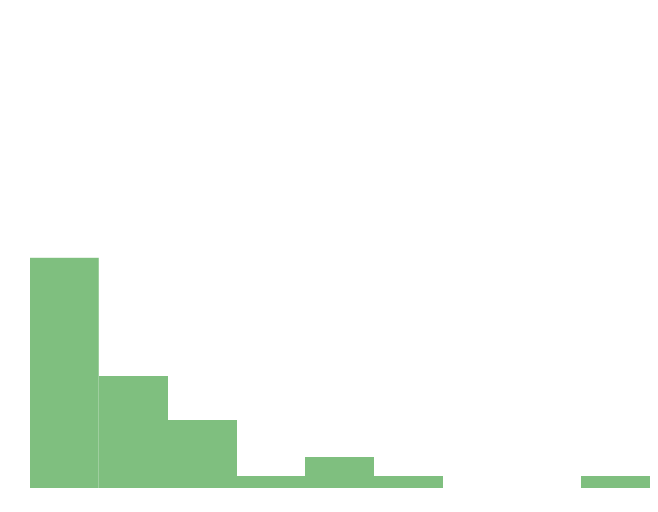
\includegraphics[width = 2cm, height = 0.5cm]{tex-inputs/table-images/voicebasedemotiondetectionben} \\ 
Facial Detection & 20.0 & 10.0 & 34.0 & 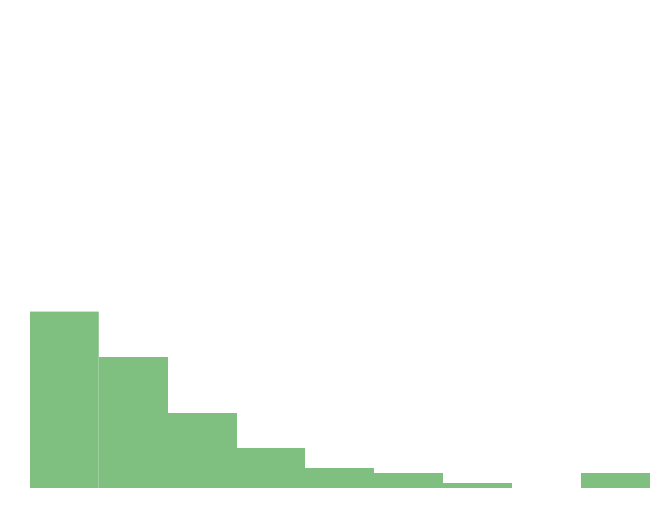
\includegraphics[width = 2cm, height = 0.5cm]{tex-inputs/table-images/facialdetectionben} \\ 
Discreet Video Camera & 20.0 & 15.0 & 30.0 & 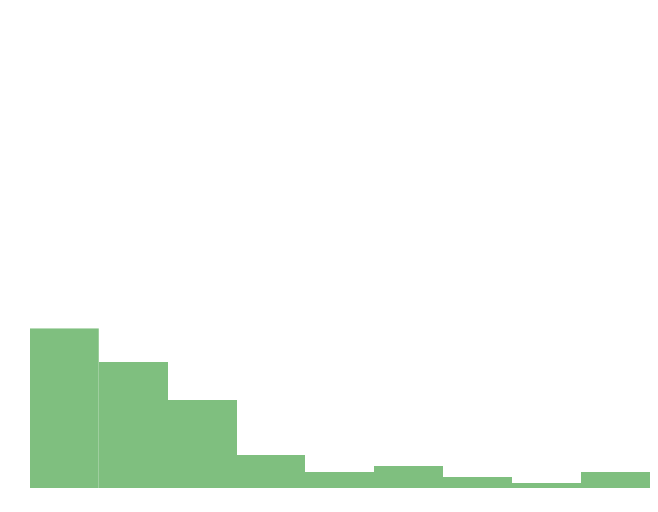
\includegraphics[width = 2cm, height = 0.5cm]{tex-inputs/table-images/discreetvideocameraben} \\ 
Google Glass & 20.0 & 12.0 & 40.0 & 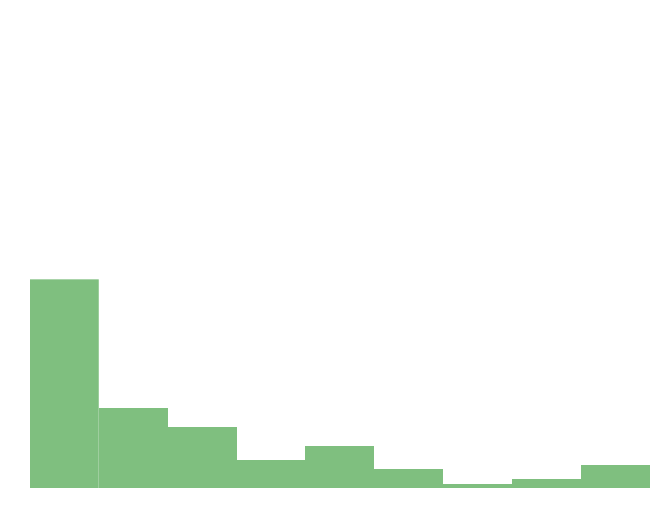
\includegraphics[width = 2cm, height = 0.5cm]{tex-inputs/table-images/googleglassben} \\ 
Smartwatches & 20.0 & 10.0 & 35.0 & 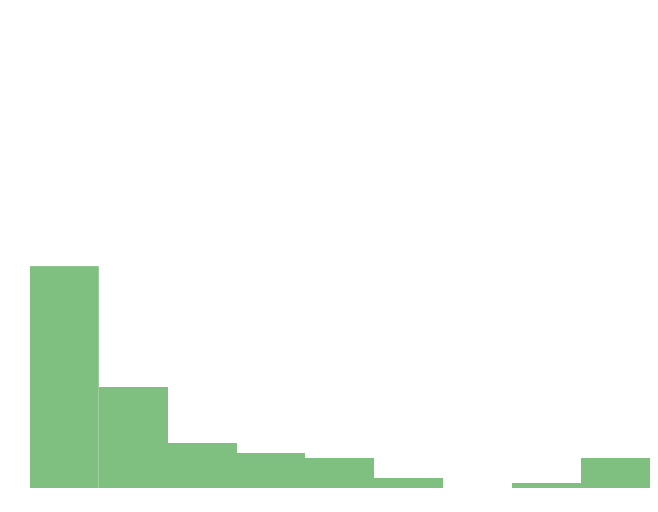
\includegraphics[width = 2cm, height = 0.5cm]{tex-inputs/table-images/smartwatchesben} \\ 
Motorcycle & 20.0 & 12.0 & 40.0 & 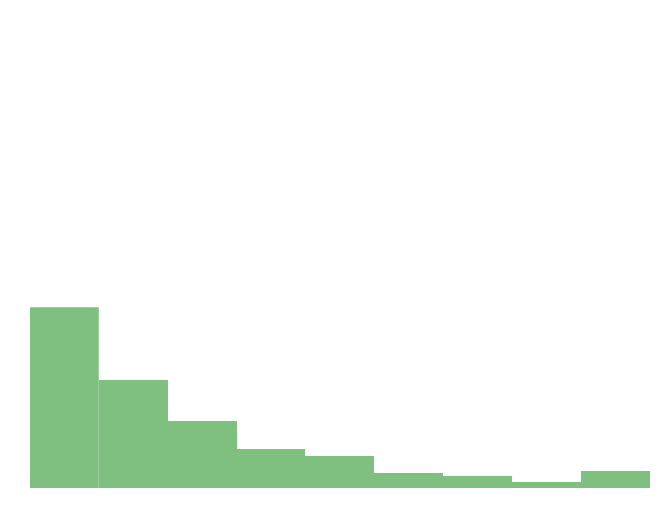
\includegraphics[width = 2cm, height = 0.5cm]{tex-inputs/table-images/MotorcycleBenefit} \\ 
Handgun & 20.0 & 10.0 & 30.0 & 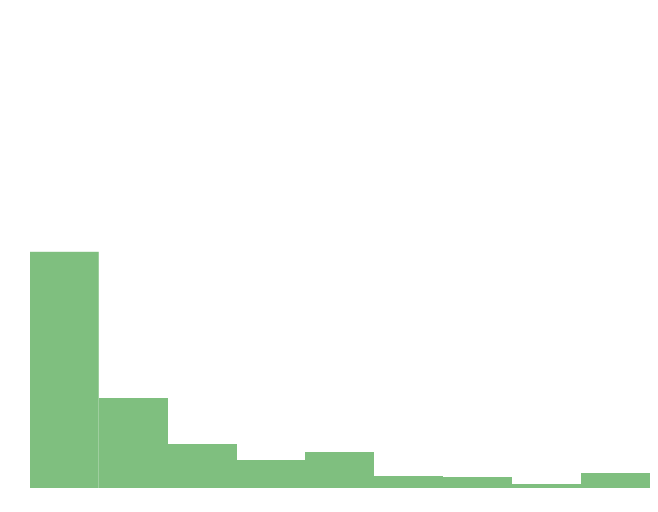
\includegraphics[width = 2cm, height = 0.5cm]{tex-inputs/table-images/HandgunBenefit} \\ 
Facial Recognition & 22.0 & 12.5 & 42.5 & 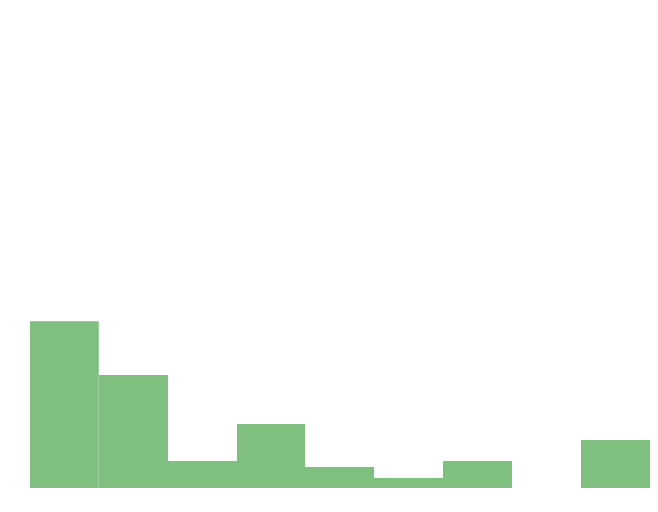
\includegraphics[width = 2cm, height = 0.5cm]{tex-inputs/table-images/facialrecognitionben} \\ 
Lawnmower & 24.0 & 15.0 & 40.0 & 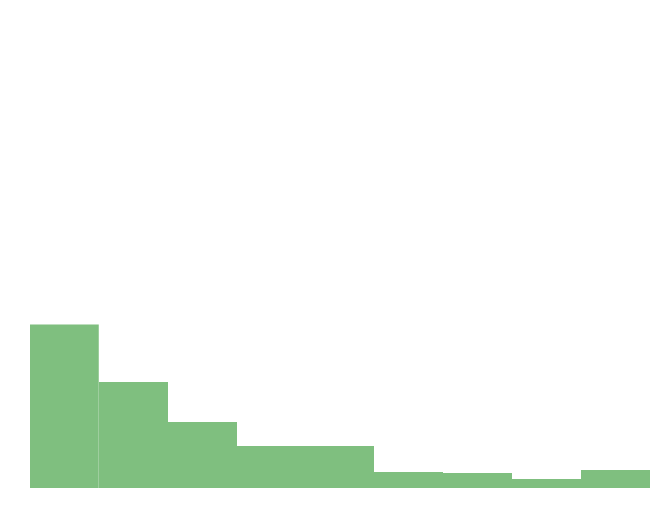
\includegraphics[width = 2cm, height = 0.5cm]{tex-inputs/table-images/LawnmowerBenefit} \\ 
Speech To Text & 25.0 & 15.0 & 40.0 & 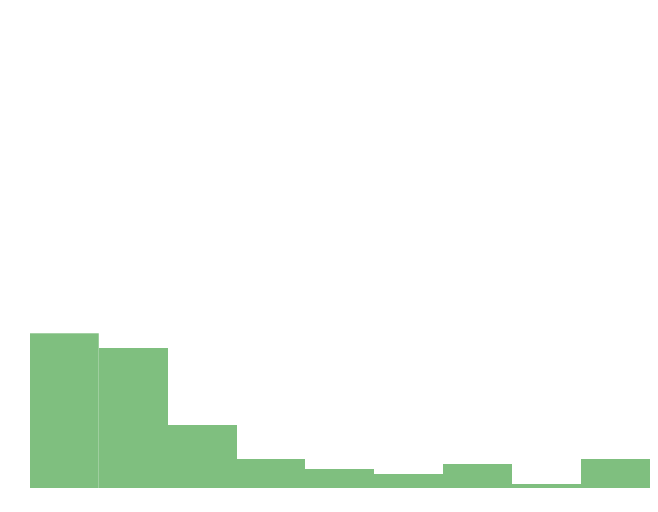
\includegraphics[width = 2cm, height = 0.5cm]{tex-inputs/table-images/speechtotextben} \\ 
Voice Recognition & 25.0 & 15.0 & 40.0 & 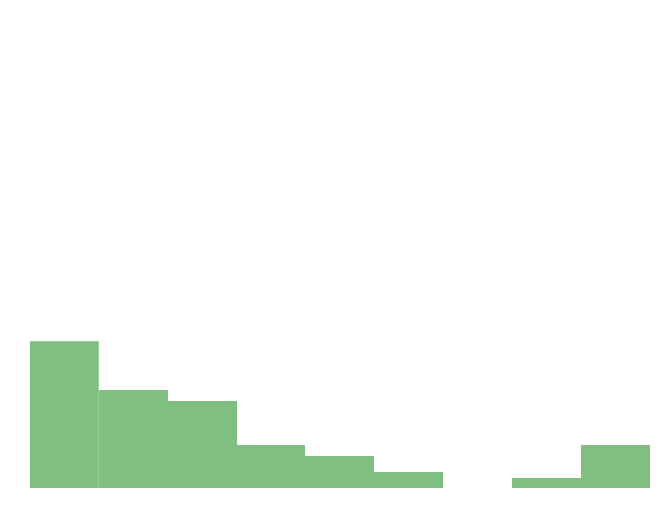
\includegraphics[width = 2cm, height = 0.5cm]{tex-inputs/table-images/voicerecognitionben} \\ 
Language Detection & 35.0 & 15.0 & 60.0 & 
\includegraphics[width = 2cm, height = 0.5cm]{tex-inputs/table-images/languagedetectionben} \\ 
Heart Rate Detection & 40.0 & 26.0 & 65.0 & 
\includegraphics[width = 2cm, height = 0.5cm]{tex-inputs/table-images/heartratedetectionben} \\ 
Location Tracking & 40.0 & 20.0 & 70.0 & 
\includegraphics[width = 2cm, height = 0.5cm]{tex-inputs/table-images/locationtrackingben} \\ 
Email & 50.0 & 29.0 & 77.5 & 
\includegraphics[width = 2cm, height = 0.5cm]{tex-inputs/table-images/emailben} \\ 
Smartphones & 50.0 & 30.0 & 75.0 & 
\includegraphics[width = 2cm, height = 0.5cm]{tex-inputs/table-images/smartphonesben} \\ 
Laptops & 60.0 & 40.0 & 80.0 & 
\includegraphics[width = 2cm, height = 0.5cm]{tex-inputs/table-images/laptopsben} \\ 
Internet & 65.0 & 45.0 & 100.0 & 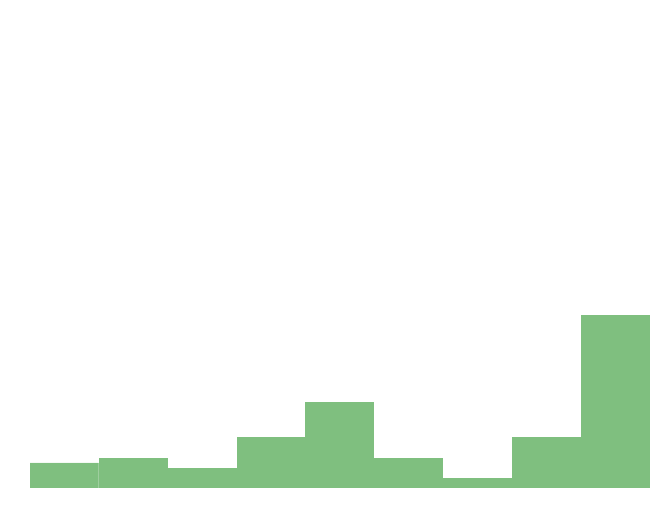
\includegraphics[width = 2cm, height = 0.5cm]{tex-inputs/table-images/internetben} \\ 
Electricity & 88.0 & 50.0 & 100.0 & 
\includegraphics[width = 2cm, height = 0.5cm]{tex-inputs/table-images/ElectricityBenefit} \\ 
\hline
\end{tabular}
\caption{Benefit rankings in response to the Fischoff-style prompt for various technologies and capabilities. Most technologies are capabilities with respect to wearable devices. Calibration technologies were electricity, guns, lawnmowers, and motorcycles. Wearable technologies included the Google Glass and the Cubetastic3000. Other specific technologies, such as internet, email, laptops, and smartphones, were also asked. }
\label{benefit}
\end{center}
\end{table}